\section{Preparing the four target core states}
\label{sec:seeds}

A seed selects an initial configuration, not a constrained solution sector.
All nine complex components subsequently relax; the driver name
\code{benchmark_axisymmetric_core_2d} does not impose cylindrical symmetry.
Its circular active mask is compatible with non-axisymmetric states. A
quadrupole seed may evolve into another core; metastability requires a
converged solution and eventually a free-energy or stability analysis.

\subsection{Exact historical and quadrupole presets}

The common initializer is \code{historical_core_seed_2d}. Define
\begin{equation}
 \ell=\frac{1}{\sqrt{1-t^2}},\qquad
 u=\frac{r}{3\ell},\qquad
 D(r)=\Delta_B\frac{\tanh u}{u},\qquad
 B(r,\phi)=\Delta_B\tanh u\,e^{\ii\phi},
 \label{eq:seed-envelope}
\end{equation}
with $D(0)=\Delta_B$ and $B(0)=0$. These are code-length seed envelopes,
not a fitted coherence length or a solution of the gap equation. Only the
historical double-core preset rescales $\ell$ by $(1+a_{\rm FL})$, using the
\emph{transformed} feedback parameter in \eqref{eq:diagonalshift}, not raw
$F_1^s$. Every preset starts with $A=B\mathbf 1_3$ and adds the following
core terms; unspecified additions are zero, and initially $\bm v=0$.

\begin{longtable}{p{29mm}p{111mm}}
\toprule
Preset & Added Cartesian components\\
\midrule
\endhead
\code{historical_nop} & None. All components vanish at the origin (normal core).\\[2mm]
\code{historical_aop} &
$A_{zx}=-A_{xz}=\tfrac{D}{2}(1+e^{2\ii\phi})$;\newline
$A_{zy}=-A_{yz}=\tfrac{\ii D}{2}(1-e^{2\ii\phi})$.\\[2mm]
\code{historical_dop} &
$A_{zx}=-A_{xz}=D\cos^2\phi$; $A_{zy}=A_{yz}=0$.
The initial shape is not a pair of prescribed, separated half cores.\\[2mm]
\code{historical_qop} &
$A_{zx}=-A_{xz}=D$; $A_{zy}=-\ii D$, $A_{yz}=+\ii D$.
This is the new non-winding quadrupole filling, not a transcription of an
old \code{qop} routine.\\
\bottomrule
\end{longtable}

The old A and double-core formulas are transcribed literally. At the origin
the code chooses $\phi=0$; their angular core terms should not be mistaken
for analytically smooth continuum solutions there. Relaxation and spatial
refinement remain necessary. The quadrupole filling is angle-independent and
finite at the origin. Before the first map, dependent halo nodes are rebuilt
from the chosen seed using the common asymptotic policy.

\subsection{Harmonics and the quadrupole phase distinction}

The diagnostic basis has spin/orbital indices in the order $(+,0,-)$. In
particular,
\begin{equation}
 C_{0\pm}=\frac{A_{zx}\mp\ii A_{zy}}{\sqrt2},\qquad
 C_{\pm0}=\frac{A_{xz}\mp\ii A_{yz}}{\sqrt2}.
\end{equation}
The historical A seed contains
$C_{0+}=D/\sqrt2$, $C_{0-}=De^{2\ii\phi}/\sqrt2$ and
$C_{+0}=-C_{0+}$, $C_{-0}=-C_{0-}$.
The historical double-core filling has
$C_{0+}=C_{0-}=D\cos^2\phi/\sqrt2$ with opposite $C_{\pm0}$.
For the new quadrupole seed,
\begin{equation}
 C_{0-}=\sqrt2D,\qquad C_{-0}=-\sqrt2D,\qquad
 C_{0+}=C_{+0}=0.
 \label{eq:quadrupole-seed}
\end{equation}
These are full local harmonic amplitudes. In particular, the occupied
quadrupole core terms have \emph{no} extra angular phase factor.

When embedding an axisymmetric radial reference, the separate symmetry rule
is $C_{\mu\nu}(r,\phi)=C_{\mu\nu}(r,0)
e^{\ii(N-\mu-\nu)\phi}$. Applying it to \eqref{eq:quadrupole-seed}
would incorrectly attach $e^{2\ii\phi}$. Neither that embedding rule nor any
radial rotational constraint is applied to the relaxed full 2D state.

The radial/2D comparison also exposed a historical inverse-transform error.
The general inverse contains
\begin{equation}
 A_{xy}=\frac{\ii}{2}(C_{++}-C_{--}+C_{-+}-C_{+-}).
\end{equation}
The old sign choice for the first two terms artificially imposed
$A_{xy}=-A_{yx}$. The working radial source and physical 2D embedding now
use the corrected inverse. A deliberately named legacy-transport projection
remains only for archival compatibility comparisons; those tests must not
be confused with the corrected physical reference.

\begin{landscape}
\begin{figure}[p]
\centering
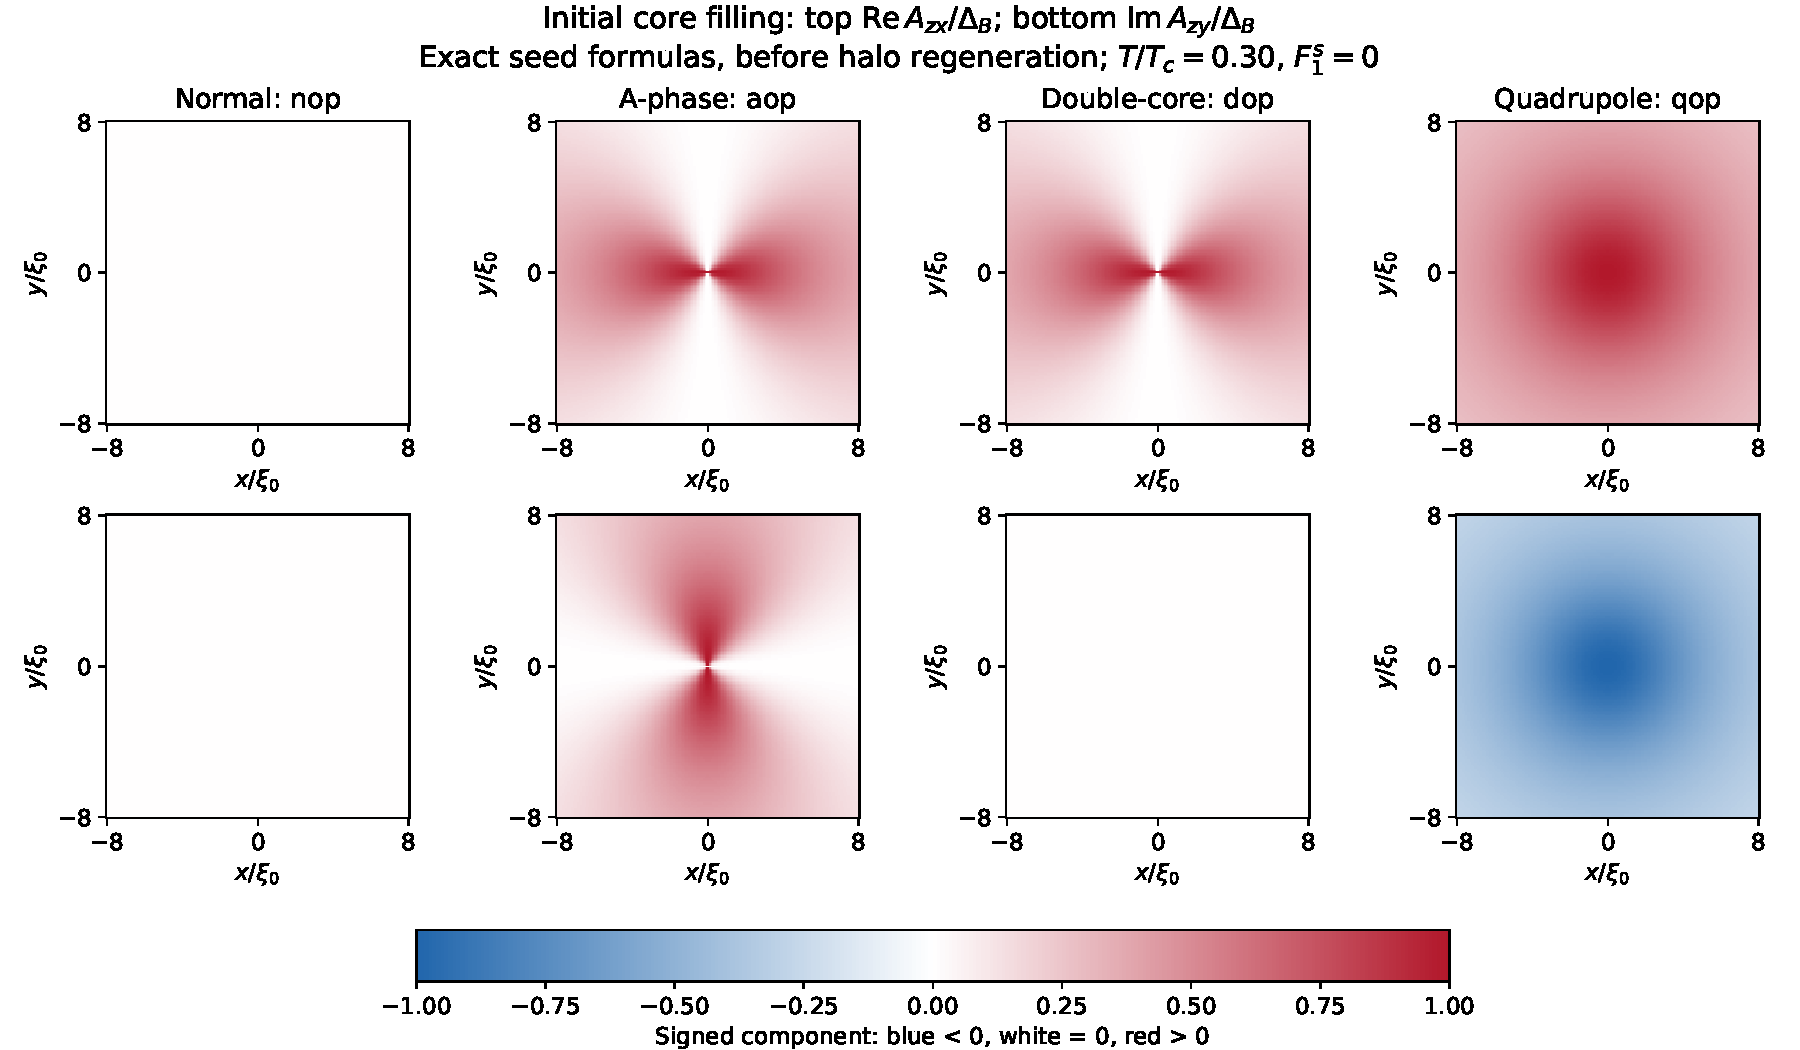
\includegraphics[width=\linewidth,height=122mm,keepaspectratio]{figures/core_initializations.pdf}
\caption{Two signed Cartesian components distinguish the four initializers.
The common diagonal phase-wound background is omitted from the panels.
All panels share the same amplitude scale; blue is negative, white is zero,
red is positive. These are exact initializer formulas at $t=0.30$, $F_1^s=0$,
not relaxed solutions. The $\cos^2\phi$ structure in the historical A and
double-core seeds and the non-winding quadrupole filling are intentionally
shown without smoothing or reinterpretation.}
\label{fig:core-seeds}
\end{figure}
\end{landscape}

\subsection{Reference, restart and core transfer are different operations}

\code{radial_reference} embeds a saved radial profile; \code{restart} reads
a dense 2D field on the identical mesh and resets Anderson history.
\code{restart_core} first embeds the specified radial reference on the new
mesh and then copies exact old nodes inside \code{restart_core_radius}.
It is useful with \code{extended_smooth}, whose inner coordinates are
preserved, but is not arbitrary remeshing and must not silently interpolate a
checkpoint. Imported legacy double-core fields and the regularised London
double-core model remain separate options in the double-core workflow.
